\chapter{Concepts and Architecture}

\section{General overview}
How all components are connected to each other (cineast, feature module, cottontail, rest api, polygonizer, voxel storage, vr interaction controller, etc.)

\section{Cineast}
What is cineast, how does it work (feature modules, cottontail etc.)...

\subsection{Extraction Modules}
What, how

\subsection{Queries}
What, how, KNN, etc.

\section{Voxels}
What are voxels, purpose, hermite data, etc.

\newpage
\section{Isosurface Polygonization}

\begin{wrapfigure}{R}{0.25\textwidth}
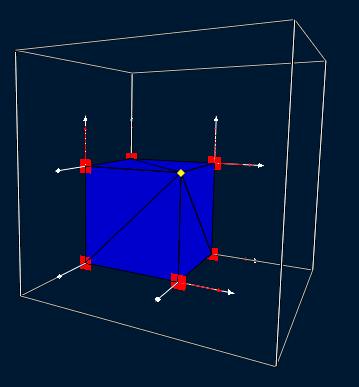
\includegraphics[width=0.25\textwidth]{voxel_scene_cube.png}
\caption{A polygonized voxel cell (white) containing the polygon surface of a cube's corner (blue) with a sharp feature (yellow).}
\label{fig:polygonized_cube_voxel_cell}
\end{wrapfigure}

%Method for converting voxels into meshes, some common algorithms as examples

There are two main groups of such algorithms: primal (\todoMissing{Missing ref; MC etc.}) and dual (\todoMissing{Missing ref; DC, CMS, etc.}) contouring algorithms.
Generally these algorithms cannot polygonize a single voxel by itself, but instead require a cell consisting of eight voxels, usually arranged in the form
of a cube. Primal and dual contouring algorithms differ in that the primal variants place polygon vertices somewhere on the cell's edges and the dual variants
place them not on the edges but somewhere within the cell's volume. Therefore dual contouring algorithms have the advantage that they can more reliably polygonize
surfaces with sharp features, such as e.g. the corners of a cube. Primal contouring algorithms can also polygonize sharp features in certain cases, however only
if said sharp feature lies exactly on a cell's edge. Fig. \ref{fig:polygonized_cube_voxel_cell} shows a polygonized voxel cell where the sharp feature lies within
the voxel cell.\\
Marching Cubes [\todoMissing{Missing ref}] (MC), a primal contouring algorithm, checks whether the material at each corner of the voxel is filled or empty and then 
packs all 8 resulting booleans into a single 8 bit integer. That integer is then used to index into a lookup table that contains which cell edges are to be connected to
each other to form polygons. Vertex positions can either lie on the middle of their respective cell edge or if the voxel contains a density value the vertex position
can be smoothly linearly interpolated.\\
Dual Contouring [\todoMissing{Missing ref}] (DC) uses another approach. A valid voxel cell always contains either no edge with a material, or at least three edges with a material change. If a voxel cell
does contain edges with a material change then Dual Contouring finds the sharp feature that minimizes the squared distance between the sharp feature and all planes spanned
by the normals at the edges with the material changes. In a second pass the generated vertices are then connected between neighboring voxel cells to form polygons.\\
Cubical Marching Squares [\todoMissing{CMS}] (CMS) makes use of both primal and dual contouring features. Much like MC it places vertices on voxel cell edges. However it can also place vertices
on voxel cell faces and within the voxel cell volume, like dual contouring algorithms do. This gives it the advantage that each cell can be polygonized individually while still being able to
reliably polygonize surfaces with sharp features.

\section{CSG}

\begin{figure}
\centering
\captionsetup{width=0.4\textwidth}
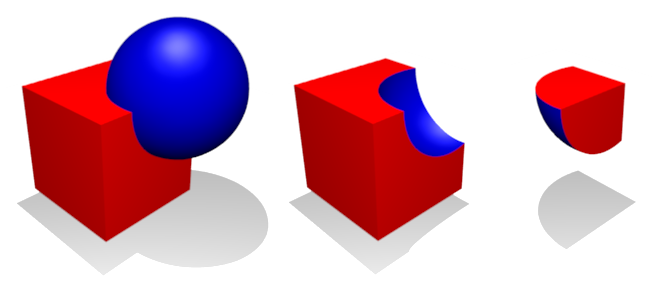
\includegraphics[width=0.4\textwidth]{csg_operations.png}
\caption{Boolean union (left), difference (middle) and intersection (right) of a cube and sphere primitive. Adapted from Wikipedia\protect\footnotemark.}
\label{fig:csg_operations}
\end{figure}
\footnotetext{\url{https://en.wikipedia.org/wiki/Constructive_solid_geometry}}

Constructive Solid Geometry (CSG) is a method to create geometric shapes by constructing them from primitives and a few operations.
The three most common operations are the boolean union ($\cup$), difference ($-$) and intersection ($\cap$) operations are shown in Fig. \ref{fig:csg_operations}. With just
those three simple tools and a couple of primitives, e.g. spheres, cubes, cylinders, etc., the user can easily create arbitrary shapes or sculptures.
Additionally CSG need not be restricted to only boolean operations, but can also make use of smooth operations that blend two shapes together in a continuous
manner. In the context of signed distance functions (see further below) these smooth operations correspond to the smooth minimum and maximum operations.\\
The application developed for this thesis makes extensive use of CSG to enable the users to edit and shape their voxel based sculptures. The union ("add") and
difference ("remove") operations are intuitive and easy to use. Additionally it also provides a "replace" operation that allows the user to replace solid materials inside
a primitive with another material. Logically it is equivalent to $(A-B) \cup (B \cap A)$ where A is the existing sculpture and B is the primitive or bounds within
which solid materials should be replaced with B's material.

\section{Signed Distance Functions}

Signed distance functions (SDF) are mathematical formulas that describe the signed distance between a point and the surface of a certain shape. For points inside the shape the
signed distance is negative. For example it is trivial to derive the signed distance function $f(x,y,z) = \sqrt{x^2 + y^2 + z^2} - r$ of a sphere at $(0, 0, 0)$ from the implicit formula of the sphere's surface, $x^2 + y^2 + z^2 - r^2 = 0$. There exist readily available formulas for SDFs of various shapes, e.g. Inigo Quilez' collection of such functions\footnote{\url{https://iquilezles.org/www/articles/distfunctions/distfunctions.htm}}.\\
SDFs are well suited as a representation of CSG primitives because one can approximate their union and difference by taking the minumum, respectively maximum, of two SDFs. This approach generally works
well and can produce the exact union or difference, however in certain cases it can result in an incorrect approximation, especially on the inside of union'd SDFs. For the purposes of this application the
SDFs need not be exact on the inside, hence we have decided to use SDFs as the representation of our CSG primitives. Additionally since the domain and range are the same for all SDFs, namely
$f\colon \mathbb{R}^3 \mapsto \mathbb{R}$, they can all be treated exactly the same besides their formulas and can be encapsulated as a simple method in code.

\section{Voxelization}

\begin{wrapfigure}{R}{0.5\textwidth}
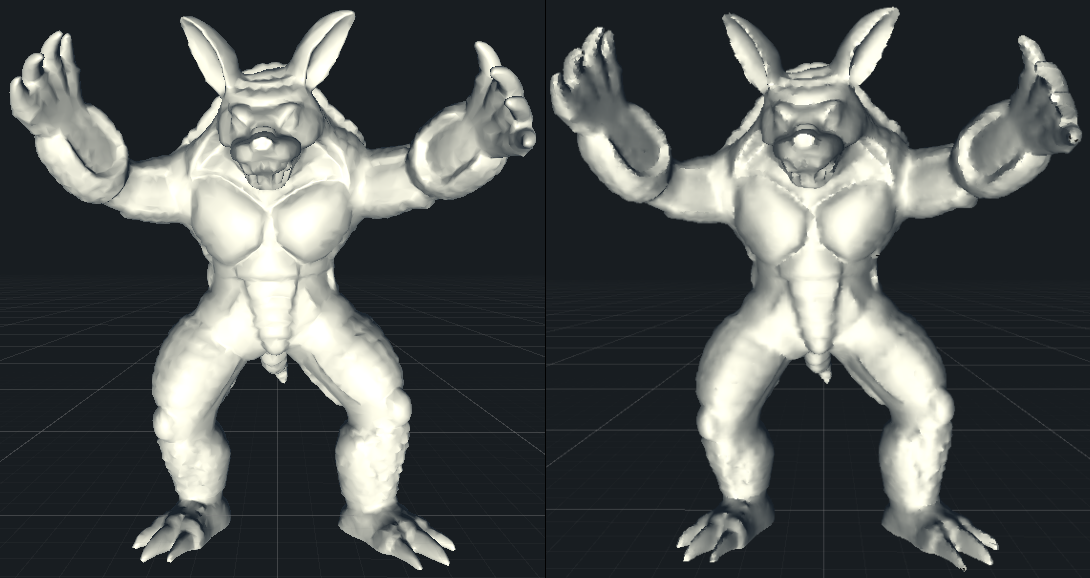
\includegraphics[width=0.5\textwidth]{voxelizer_example.png}
\caption{The Stanford Armadillo mesh\protect\footnotemark  (left) and its voxel representation at a resolution of 128x128x128 voxels (right).}
\label{fig:voxelizer_example}
\end{wrapfigure}
\footnotetext{\url{http://graphics.stanford.edu/data/3Dscanrep/}}

An important part of multimedial retrieval is the ability to take query results and reuse them to formulate a new query. In the context of this thesis the multimedia retrieval
is only concerned with polygonal meshes. To facilitate the modification of such polygonal meshes the application includes a voxelizer module. A voxelizer takes a polygonal
mesh as input and converts it into a suitable voxel representation. In particular, to achieve high accuracy our voxelizer converts the polygonal mesh into Hermite data. Since
Hermite data contains not only the voxel material, but also the surface normals, we can reconstruct the mesh from the Hermite data voxels while keeping most of the mesh's features intact, given
a large enough voxel grid with sufficient resolution. In practice a resolution of 128x128x128 seems to be sufficient for most models that aren't highly detailed or noisy.
Fig. \ref{fig:voxelizer_example} shows an example of a mesh that has been converted to a Hermite data voxel grid.

\section{Virtual Reality}
What is VR, use cases

\subsection{UI Design}
Windows vs. using 3D space

\subsection{Sculpting interactions}
One hand to grab, other to sculpt, rotating brush with trackpad, etc.

\section{Unity}
What, why